

\documentclass[journal]{IEEEtran}

\usepackage{graphicx}
\usepackage{url}
\begin{document}


\title{Development of a Human Movement Codec}
% Compression of Kinematic Data
% Compression of Human Movement Data

\author{David~Chiasson}

\maketitle

\begin{abstract}
Real-time kinematic data is central to many emerging technology applications, yet to date few techniques have been proposed to process and represent with this relatively new information modality in an efficient manner. This paper explores techniques for the compression of human kinematic data. Techniques from traditional multimedia networks are compared with several novel approaches. Simple, computationally cheap techniques are shown to losslessly compress kinematic data by over a factor of ten compared with traditional representations. Furthermore, these simple techniques are shown to be superior to more complex approaches.
All techniques discussed in this study are implemented and released as open source code which can be quickly integrated into a variety of computational platforms. 
\end{abstract}

\begin{IEEEkeywords}
kinematic data, human movement, compression, codec
\end{IEEEkeywords}



\section{Introduction}

\IEEEPARstart{M}{any} emerging technology applications rely on on real-time kinematic data as a crucial component. These include virtual reality, autonomous driving, internet of things, physical therapy, wearable electronics, and human performance among others. These applications have been enabled by the recent explosion of cheap inertial based sensors (IMUs) along with mobile computation power to process this data at high sampling frequency. Kinematic data represents a nascent field of multimedia data which is starkly under-developed compared to the existing maturity of text, audio, and visual type data processing techniques. In order to enable the modern applications listed above, efficient and standard techniques for representing and processing kinematic data are needed.

This study explores a range of both traditional and novel compression techniques applied to human kinematic data gathered by 6-axis IMUs. The best performing techniques are identified and discussed. Only lossless compression techniques are considered. The reason for this is that lossy compression inherently involves a value judgment about what information is useful and what information is irrelevant. In the absence of a specific application, no justification can be made for discarding any portion of information.

This study focuses on highly practical approaches which can be used in modern applications. To demonstrate this, all compression techniques have been implemented and released as open-source C code using fixed point computations. The hope of the authors is that this code can be a starting point for academic or industry developers implementing some kinematic data application on any type of computational platform.

All compression algorithms can be divided into two phases, modeling and coding[TO CITE] as shown in figure \ref{fig:general_compressor}. The model incorporates our knowledge about the signal to be compressed. It computes a probability mass function (PMF) which is an estimated likelihood of all possible input symbols. A dynamic model is one which changes its PMF estimate after new input symbols are received. The coder then reads the uncompressed data and uses the PMF to choose a unique code for each input symbol. Short codes are chosen for likely symbols and long codes are chosen for unlikely symbols such that the total length of the compressed data is minimized. The decompressor uses an identical model to provide the same PMF to the decoder which is used to revert each code back into the original symbol. If the model is dynamic, this output is used to update the model for future predictions. Coding is a solved problem and will thus not be discussed in this work.[TO CITE] Modeling on the other hand has been proven unsolvable and must be revisited for each new class of signal.(due to the pidgeon hole principal?)[TO CITE]. To the author's knowledge, no previous work has directly addressed the modeling problem for kinematic data signals. This provides the motivation for the current work. Modeling has been shown to be equivalent to the artificial intelligence problem [TO CITE].

Since the theoretical limit on the compression provided by the coder is set by Shannon's entropy law
$$H = -\sum_{i} P_ilogP_i$$
[to cite]

The goal of the model is to produce an accurate PMF with minimum entropy. Intuitively this means that compression is higher the more "sure" the model is about some occurrences over other ones. If an optimal encoder is used, the compression ratio can be regarded as a quantitative measurement of the model's understanding of the underlying signal. Because of this, we expect the performance of various signal models to give us insight into the content of the kinematic signal.

TODO: why do we assume our signal is geometrically distributed about the mean!?
TODO: relationship for natural signals of residual signal and compression ratio

In this work, the maximum likelihood occurrence according to the model will be referred to as the prediction. The difference between the prediction and the actual sample will be referred to as the residual. For practical implementation, it is advantageous to convert the original signal into the residual signal before coding so that the coder can be computationally optimized to compute encodings for zero mean random variables (or same distribution? not recalculating ).

Define stream? node? anything else?

\begin{figure}
  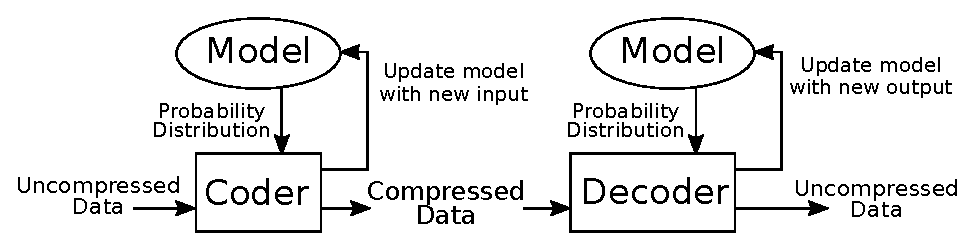
\includegraphics[width=\linewidth]{general_compressor.eps}
  \caption{General compressor and decompressor}
  \label{fig:general_compressor}
\end{figure}

We hypothesize that compression ratios will be comparable to those achieved in lossless audio compression. We also hypothesize that the best performing codec will utilize some cross axis correlation and be informed by physics based models.

\section{Method}
In order to meaningfully and repeatable demonstrate the performance of a compression algorithm, a public kinetic signal corpus must be selected. For this study, the Human Gait Database (HuGaDB) is used. HuGaDb is a public dataset of six-axis IMU signals collected from six different body segments of 18 healthy subjects performing 12 different movement activities[TO Cite]. This database was selected because it allowed the comparison of compression techniques across body segment, subject, and activity in addition to sensor modality.

The data collected from three random subjects was designated as training data, and only data from the remaining 15 subjects was used in our results. The training data was used to train the lasso regression of our cross-stream FIR filter discussed later.



\subsection{Reference Encodings}
As it is proven impossible to claim maximum compression [TO CITE] it is necessary to select a reference when evaluating the performance of a compression algorithm. In this study, the baseline encoding (exhibiting a compression ratio of one) is comma separated value (CSV), a simple text based format which is the de-facto standard for storing sensor information. Performance is compared by computing the compression ratio CR relative to CSV via the following formula:
$$CR = \frac{\textrm{size of CSV file}}{\textrm{size of compressed file}}$$
To give further context to performance, established algorithms from both text and audio compression are applied to the kinematic data. In total, the following five reference encodings are used to give context to compression ratios:

\begin{itemize}
  \item \textbf{CSV} Standard text based format. To minimize variance in csv size, each data point is formatted to the the same text length resulting in a file size of sixteen bytes per sample.
  \item \textbf{Binary} The optimal fixed size format. In our corpus, every sample is two bytes. This would be the optimal compression if each sample were an IID random variable uniformly distributed across all possible sample readings.
  \item \textbf{Binary Rice Encoded} Binary files with Rice-Golomb encoding[TO CITE] applied. This would be the optimal compression if each sample were an IID Laplacian distributed random variable with mean zero.
  \item \textbf{ZIP compression of CSV} ZIP is a general purpose compressed file format integrated into all major computer systems. [TO CITE] ZIP was executed using the DEFLATE to cite] method and a compression level of 6.
  \item \textbf{FLAC compression of binary} FLAC is a popular, open-source lossless audio codec (include options)[TO CITE]. FLAC was executed using the linear predictive coding [TO CITE] technique and a compression level of 5.
\end{itemize}
\subsection{Tested Encodings}

TODO: can I prove that the optimal IIR linear filter cannot exceed that of the optimal FIR linear filter?

Several restrictions are placed on the algorithms considered in this study. First, a viable algorithm must be causal. This is a basic requirement for an algorithm to be real-time. We also chose to only consider algorithms with zero filter delay. Since our sensors operate at a relatively low sampling frequency of 60Hz, a delay of one sample would be 16ms which is significant for modern information networks.

We also only consider algorithms which are node independent. The model for each signal considers at most the information from the six co-located signals including it's own past input. While it is likely that utilizing inter-node correlation could produce better compression ratios, especially if a human biomechanics model is introduced, such an approach would limit the usefulness of said algorithm to that specific placement of nodes on the body.

Finally, only lossless algorithms are considered. As discussed in the introduction, a lossy algorithm requires an objective metric for determining how much data loss and of what type is acceptable. Without this metric it is trivial to create a compression algorithm with an infinite compression ratio but which looses all information.

In practice, the implementation of a strictly lossless algorithm turns out to be non-trivial. This is because the industry standard for for floating point computation IEEE 754 [TO CITE] is not sufficiently stringent to guarantee identical results on various implementations [TO CITE]. Additionally, a compiler or interpreter which processes the source code for an algorithm implementation will often utilize mathematical properties such as commutativity to optimize computation. This may result in different machines performing floating point operations in a different order which could lead to differing results even if each rounding operation were well defined by IEEE 754. In order to avoid both of these scenarios and guarantee identical results across any computer, all algorithms in this study are implemented using only integer operations and fixed-point 16.16 precision.[cite fixed point math library?] There is significant cost associated with this technical decision. Namely every computation has the same distribution of rounding error independent of its magnitude. This can lead to significant numerical issues for complex algorithms [TO CITE]. In the context of compression, complex or numerically unstable algorithms may produce compression ratios which underestimate their understanding of the underlying signal since their implementation is not equivalent to their mathematical derivation.

The following encodings are implemented and discussed in this study:

\begin{itemize}
  \item \textbf{Delta encoding} Current sample is predicted to be equivalent to the previous sample so that the difference between the two is encoded. If a signal varies slowly with time, this signal will be smaller than the original signal.
  \item \textbf{Linear extrapolation} Current sample is estimated as a linear extrapolation from previous samples. Also known as first order polynomial regression.
  \item \textbf{\boldmath$2^{nd}$ to \boldmath$5^{th}$ order polynomial regression} This technique assumes that the signal is a polynomial which is estimated from a least squares regression of past samples. This polynomial is then extended to get a prediction of the current sample.
  \item \textbf{Spline extrapolation} A spline is the minimum curvature piece-wise polynomial which connects a set of points. It is commonly used for interpolation, namely computer graphics smoothing. This technique was selected as splines are known to avoid Runge's phenomenon which is witnessed when extrapolating higher order polynomials. Results from the cubic spline with natural boundary conditions are presented in this paper.
  \item \textbf{Linearized rotating gravity} A Newtonian physics based model in which a constant magnitude acceleration vector rotates according to gyroscope readings.
  \item \textbf{Trained auto-corrolation linear prediction} The optimal linear predictor of training data utilizing each signal's history.
   \item \textbf{Trained cross-corrolation linear prediction} The optimal linear predictor of training data utilizing all six co-located signal histories.
\end{itemize}

\subsection{Implementation}


To show algorithm performance in a realistic scenario, as well as to provide tools of benifit to the community, the algorithms in this study have been implemented in the C programming language and released as open-source code found at \url{https://github.com/dchiasson/kinetic_codec}. TODO[change the name of the repo, clean up docs, and release]. The choice of programming language as well as the restriction to integer arithmetic allow this code to be easily incorporated into programs executing on either a traditional computer or embedded computation platforms, even those without a floating-point unit.
\begin{figure}
  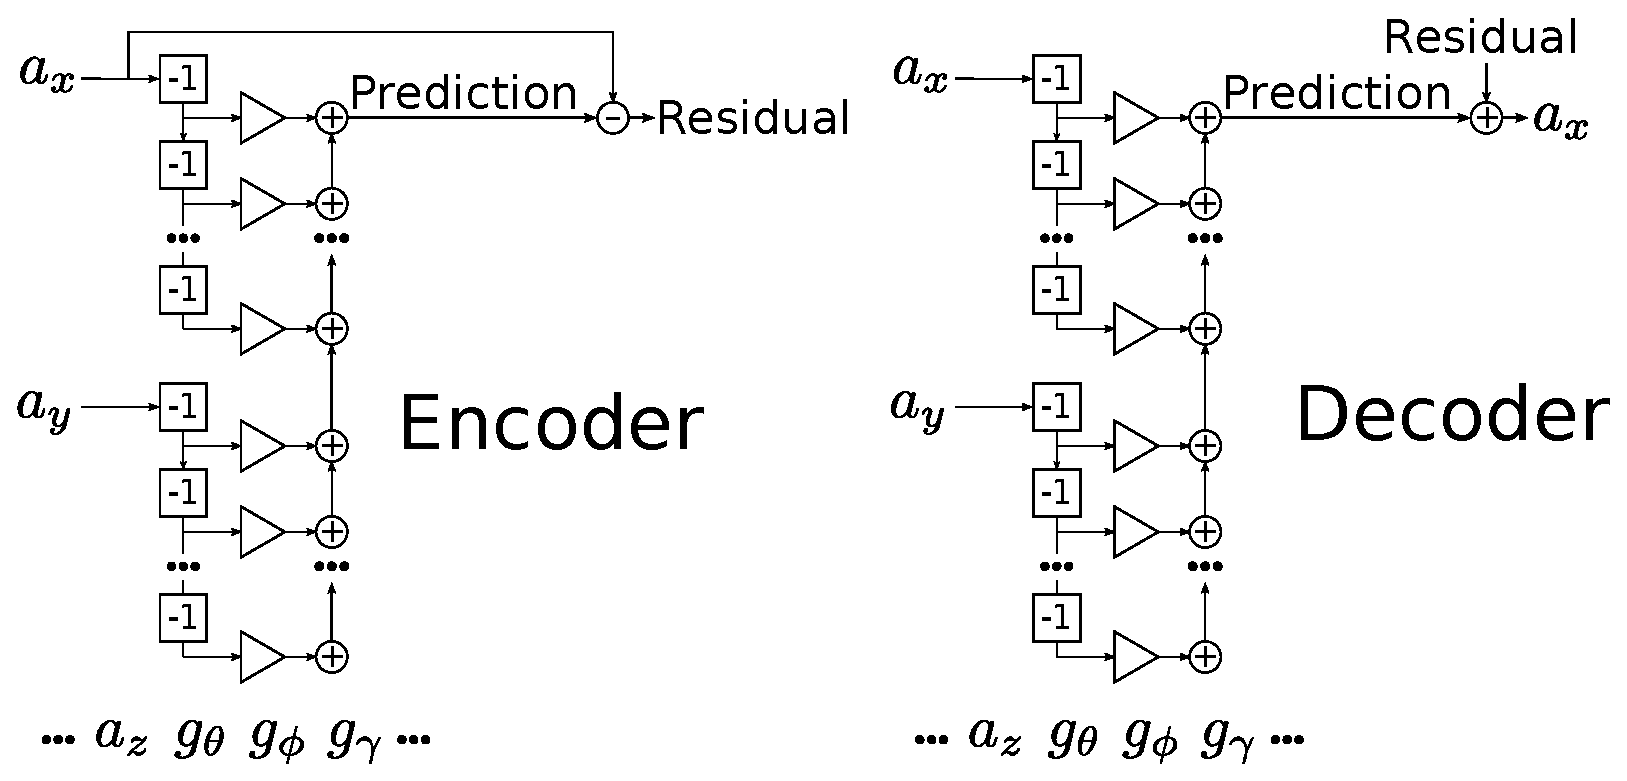
\includegraphics[width=\linewidth]{flow_diagram.eps}
  \caption{Flow diagram of encoder and decoder.}
  \label{fig:flow_diagram}
\end{figure}

Figure \ref{fig:flow_diagram} shows the computational flow chart [probably remove this]


\section{Results}


\begin{figure}

  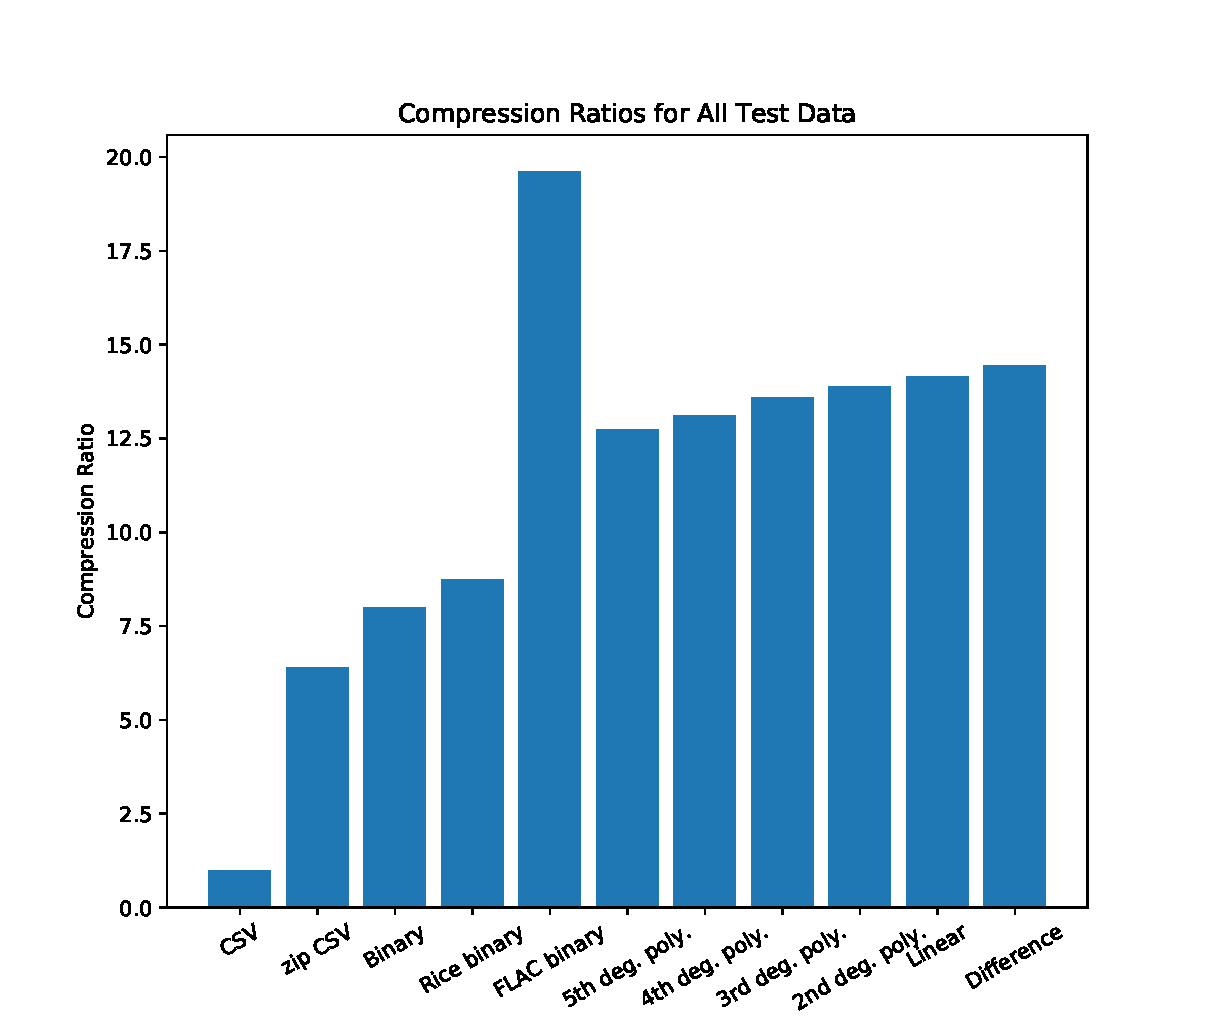
\includegraphics[width=\linewidth]{prelim_results.eps}
  \caption{Compression ratio (original size / compressed size) of each encoding technique on all test data. Larger is better.}
  \label{fig:main_results}
  
\end{figure}
\begin{figure}

  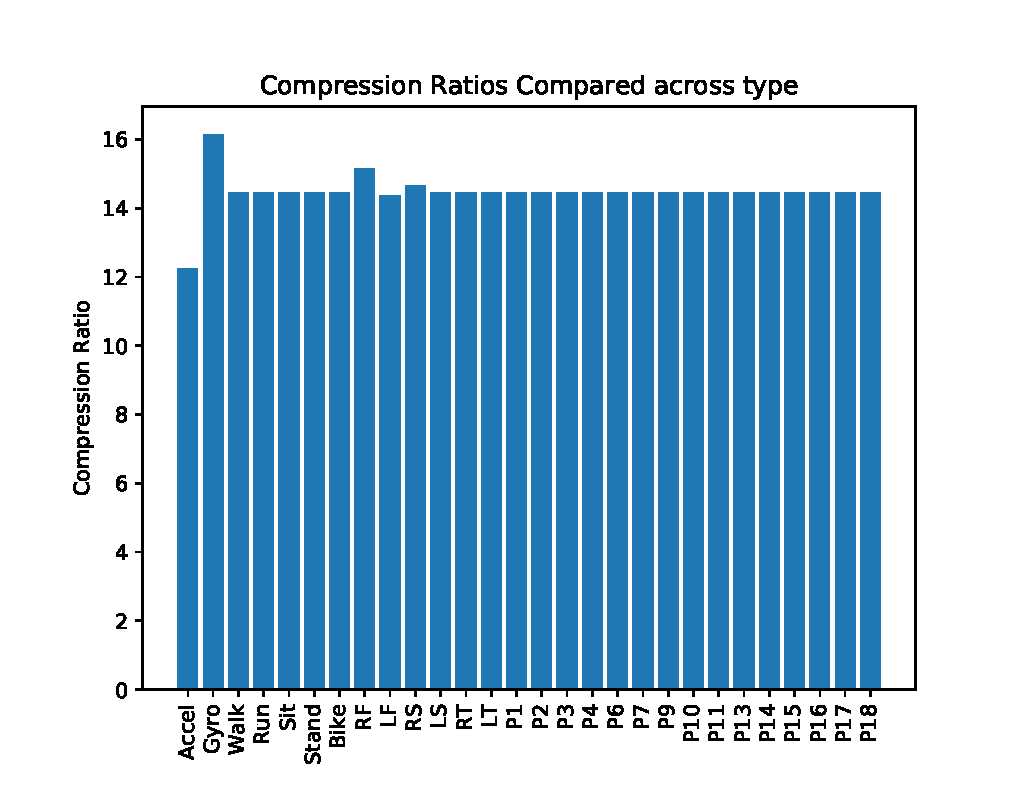
\includegraphics[width=\linewidth]{results_type_split.eps}
  \caption{Compression ratio (original size / compressed size) of each encoding technique on all test data. Larger is better.}
  \label{fig:split_results}
  
\end{figure}

\begin{table*}[]
\begin{tabular}{lllllllllllllllllllllllllllllllll}
                        &            &                &                                       & \multicolumn{5}{c}{\textbf{Activity}}                                                                             & \multicolumn{6}{c}{\textbf{Body Segment}}                                                                                              & \multicolumn{18}{c}{\textbf{Subject Number}}                                                                                                                                                                                                                                                                                                            \\
                        & \textbf{K} & \textbf{Order} & \multicolumn{1}{l|}{\textbf{All}}     & \textbf{Walk}    & \textbf{Run}     & \textbf{Sit}     & \textbf{Stand}   & \multicolumn{1}{l|}{\textbf{Bike}}    & \textbf{R. Foot} & \textbf{L. Foot} & \textbf{R. Shin} & \textbf{L. Shin} & \textbf{R. Thigh} & \multicolumn{1}{l|}{\textbf{L. Thigh}} & \textbf{1}       & \textbf{2}       & \textbf{3}       & \textbf{4}       & \textbf{5} & \textbf{6}       & \textbf{7}       & \textbf{8} & \textbf{9}       & \textbf{10}      & \textbf{11}      & \textbf{12} & \textbf{13}      & \textbf{14}      & \textbf{15}      & \textbf{16}      & \textbf{17}      & \multicolumn{1}{l|}{\textbf{18}}      \\ \hline
\textbf{CSV}            & -          & -              & \multicolumn{1}{l|}{1}                & 1                & 1                & 1                & 1                & \multicolumn{1}{l|}{1}                & 1                & 1                & 1                & 1                & 1                 & \multicolumn{1}{l|}{1}                 & 1                & 1                & 1                & 1                &            & 1                & 1                &            & 1                & 1                & 1                &             & 1                & 1                & 1                & 1                & 1                & \multicolumn{1}{l|}{1}                \\
\textbf{zip CSV}        & -          & -              & \multicolumn{1}{l|}{6.39430101906924} &                  &                  &                  &                  & \multicolumn{1}{l|}{}                 &                  &                  &                  &                  &                   & \multicolumn{1}{l|}{}                  &                  &                  &                  &                  &            &                  &                  &            &                  &                  &                  &             &                  &                  &                  &                  &                  & \multicolumn{1}{l|}{}                 \\
\textbf{Binary}         & -          & -              & \multicolumn{1}{l|}{8}                & 8                & 8                & 8                & 8                & \multicolumn{1}{l|}{8}                & 8                & 8                & 8                & 8                & 8                 & \multicolumn{1}{l|}{8}                 & 8                & 8                & 8                & 8                &            & 8                & 8                &            & 8                & 8                & 8                &             & 8                & 8                & 8                & 8                & 8                & \multicolumn{1}{l|}{8}                \\
\textbf{Rice binary}    & 12         & -              & \multicolumn{1}{l|}{8.75550182215849} & 8.7555021779827  & 8.75551024333942 & 8.75550182215849 & 8.75550283269934 & \multicolumn{1}{l|}{8.75550315181756} & 8.6141477456608  & 8.4905694245542  & 8.96410656362444 & 8.82750916390295 & 8.82319690149691  & \multicolumn{1}{l|}{8.83066960944318}  & 8.75550225035374 & 8.75551024333942 & 8.75550330824806 & 8.75550330824806 &            & 8.75550367070901 & 8.75550302518334 &            & 8.75550182215849 & 8.75550350639338 & 8.75550330824806 &             & 8.75550315181756 & 8.75550263711077 & 8.75550182215849 & 8.75550182215849 & 8.75550367070901 & \multicolumn{1}{l|}{8.75550263711077} \\
\textbf{FLAC binary}    & 0          & 0              & \multicolumn{1}{l|}{19.6099365007281} &                  &                  &                  &                  & \multicolumn{1}{l|}{}                 &                  &                  &                  &                  &                   & \multicolumn{1}{l|}{}                  &                  &                  &                  &                  &            &                  &                  &            &                  &                  &                  &             &                  &                  &                  &                  &                  & \multicolumn{1}{l|}{}                 \\
\textbf{Spline}         & 0          & 0              & \multicolumn{1}{l|}{}                 &                  &                  &                  &                  & \multicolumn{1}{l|}{}                 &                  &                  &                  &                  &                   & \multicolumn{1}{l|}{}                  &                  &                  &                  &                  &            &                  &                  &            &                  &                  &                  &             &                  &                  &                  &                  &                  & \multicolumn{1}{l|}{}                 \\
\textbf{5th deg. poly.} & 8          & 19             & \multicolumn{1}{l|}{12.7401178924573} & 12.7402049974879 & 12.7409038571714 & 12.7401953539615 & 12.7402467059078 & \multicolumn{1}{l|}{12.7404859033232} & 13.5087448977051 & 12.782177346666  & 12.9935043898734 & 12.8920826243934 & 12.8033209307301  & \multicolumn{1}{l|}{12.6770324260121}  & 12.7402272675518 & 12.7409038571714 & 12.74031366544   & 12.74031366544   &            & 12.7402798970202 & 12.7402738084908 &            & 12.7402862899823 & 12.7403451316287 & 12.74031366544   &             & 12.7402944545802 & 12.7403347782204 & 12.7403317584795 & 12.7403035263679 & 12.7402798970202 & \multicolumn{1}{l|}{12.7403347782204} \\
\textbf{4th deg. poly.} & 7          & 19             & \multicolumn{1}{l|}{13.1118619820637} & 13.1120129435405 & 13.1132114972774 & 13.1119919557271 & 13.1120837439905 & \multicolumn{1}{l|}{13.1124890829694} & 14.4379978221238 & 13.3012440458969 & 13.5679392198626 & 13.4084547922464 & 13.0340525250709  & \multicolumn{1}{l|}{13.0602896796995}  & 13.112048326898  & 13.1132114972774 & 13.1121989310805 & 13.1121989310805 &            & 13.1121402382188 & 13.1121303670927 &            & 13.1121449368801 & 13.1122469262986 & 13.1121989310805 &             & 13.112161040367  & 13.1122374218413 & 13.1122214287952 & 13.1121789331766 & 13.1121402382188 & \multicolumn{1}{l|}{13.1122374218413} \\
\textbf{3rd deg. poly.} & 7          & 19             & \multicolumn{1}{l|}{13.5969932983155} & 13.5971381903649 & 13.5983046256314 & 13.5971201261144 & 13.5972121298592 & \multicolumn{1}{l|}{13.5975961923989} & 14.7318914460319 & 13.8744562839619 & 13.9856313282954 & 13.9407973646265 & 13.4594175347882  & \multicolumn{1}{l|}{13.5910643296974}  & 13.5971722259607 & 13.5983046256314 & 13.5973256757377 & 13.5973256757377 &            & 13.5972636085114 & 13.5972580886768 &            & 13.5972694043424 & 13.59737298708   & 13.5973256757377 &             & 13.5972883249105 & 13.5973541180008 & 13.5973440446857 & 13.5973025777271 & 13.5972636085114 & \multicolumn{1}{l|}{13.5973541180008} \\
\textbf{2nd deg. poly.} & 7          & 13             & \multicolumn{1}{l|}{13.878393070373}  & 13.8785077289018 & 13.8794193164099 & 13.8784928430834 & 13.878563302906  & \multicolumn{1}{l|}{13.8788698732695} & 14.9133016569147 & 14.0962741451877 & 14.184464741827  & 14.126332104716  & 13.7186268854952  & \multicolumn{1}{l|}{13.7910028756106}  & 13.878534641197  & 13.8794193164099 & 13.8786517240878 & 13.8786517240878 &            & 13.8786045480122 & 13.8785990922963 &            & 13.8786102765186 & 13.8786885665794 & 13.8786517240878 &             & 13.8786226380484 & 13.8786784645865 & 13.8786689939814 & 13.8786363731074 & 13.8786045480122 & \multicolumn{1}{l|}{13.8786784645865} \\
\textbf{Linear}         & 7          & 8              & \multicolumn{1}{l|}{14.1599487678905} & 14.1600319270935 & 14.16070287805   & 14.1600215034495 & 14.1600743663739 & \multicolumn{1}{l|}{14.1603025161539} & 15.06814622919   & 14.312890103988  & 14.4019085544289 & 14.3075286488473 & 14.0234735656561  & \multicolumn{1}{l|}{14.0223041569188}  & 14.1600537587462 & 14.16070287805   & 14.1601396681783 & 14.1601396681783 &            & 14.1601040213579 & 14.160100797984  &            & 14.160107405902  & 14.1601624721249 & 14.1601396681783 &             & 14.1601147093975 & 14.1601562194225 & 14.1601503575191 & 14.1601301665555 & 14.1601040213579 & \multicolumn{1}{l|}{14.1601562194225} \\
\textbf{Difference}     & 7          & 1              & \multicolumn{1}{l|}{14.4571554136452} & 14.4571827675638 & 14.4574186266642 & 14.457181748902  & 14.4571975915343 & \multicolumn{1}{l|}{14.4572703883325} & 15.1302863181696 & 14.3750749883684 & 14.4150787149968 & 14.4210188690249 & 14.4482106056356  & \multicolumn{1}{l|}{14.3506371949639}  & 14.4571892791098 & 14.4574186266642 & 14.4572196335153 & 14.4572196335153 &            & 14.4572095533327 & 14.4572065132804 &            & 14.457212745389  & 14.4572288176939 & 14.4572196335153 &             & 14.4572123828563 & 14.4572240774713 & 14.4572282436824 & 14.4572196335153 & 14.4572095533327 & \multicolumn{1}{l|}{14.4572240774713}
\end{tabular}
  \caption{This table is way to big and needs to be reformatted}
  \label{table:results}
\end{table*}


Figure \ref{fig:main_results} shows the best compression ratio of all test data for each encoding type. Delta encoding saw the highest compression of the polynomial regression techniques (CR=14.457), and each higher degree polynomial performed progressively worse with 5th degree polynomial at the bottom (CR=12.740).

Table TODO shows the breakdown of CR for each modality, activity, body segment, and subject. No significant difference was found with any algorithm for compression between subject or activity. There are minor differences across body segment and major differences between sensor modality.

TODO: quantify statistical significance

Tables of detailed results k, order: total, accel/gryo, activity, segment, subject 

TODO: Discussion of cross stream FIR coefficients, pole zero plots, precision effect
\section{Discussion}

These results show that even simple techniques result in a significant compression over the traditional encoding of CSV. If bandwidth or storage space is any concern in a kinematic data application, using a binary format would have very few disadvantages other than the loss of human-readability. Even more significant gains can be achieved with the trivial technique of delta encoding.

We were surprised by the small variation in CR across body segments, and the complete lack of variation across activity and subject. The small differences of body segments may even be due not to the differences in movement, but due to noise and bias differences between sensor hardware, as each trial had the same sensor on the same body segment(can I confirm this?). The activity and subject results average across sensor hardware, but body segment would expose any differences.

This observation, along with the surprisingly poor performance of our physics based model suggests that the information in our signal has less to do with the human body and it's movement than previously assumed. If the movement of the human body made up the vast majority of the signal content, we would expect to see significant differences in compression ratios between running and sitting. It is possible that the bulk of the entropy in our signal is due to noise, sculling and/or coning. If this is the case, it presents a significant opportunity for lossy compression algorithms to achieve significantly more compression that shown in this study.

An alternate explanation for this result may be the aliasing of the kinematic signal. 60Hz is is common for consumer grade IMUs, but it is generally agreed to be well below what is required to fully capture human movement[TO CITE]. Fast movements such as running are often sampled at 1000Hz. If the signals are significantly undersampled, we may be loosing much of the high frequency information that would differentiate fast movements from slow movements. [TODO: research effect of aliasing on information content]


Was poor performance of complex algorithms due to precision issues?

Surprising performance of difference encoding

Lack of correlation between accelerometer and gyroscope

Compression rate compared to audio

\subsection{limitations}

The compression ratios presented in this paper are intended to demonstrate the relative difference between compression techniques and may not be representative of the absolute CR experienced in other applications. There are many other factors which can affect the compression ratio which are not explored in this paper. Namely, sensor hardware differences of precision, noise, bias, and sampling rate are expected to have a large impact on the CR achieved. Additionally, CSV encoding which is used as the reference in this study, does not have a well defined size per sample. While in this study the samples were formatted to a fixed text length to preserve precision and cause deterministic size, the real size of a CSV file could vary dramatically with no upper limit depending on the formatting chosen. (should I leave that part out? I basically admitted that all my CR values are arbitrary...)

In the future, these techniques will be applied to various sensing hardware, sampling rates, and body segments.
improvements: dynamic K, blocking for error recovery

\section{Conclusion}
Kabam! Splat!


% use section* for acknowledgment
\section*{Acknowledgment}

The authors would like to thank your mom.

\begin{thebibliography}{1}

\bibitem{IEEEhowto:kopka}
H.~Kopka and P.~W. Daly, \emph{A Guide to \LaTeX}, 3rd~ed.\hskip 1em plus
  0.5em minus 0.4em\relax Harlow, England: Addison-Wesley, 1999.

\end{thebibliography}

\end{document}
